\documentclass[journal,comsoc]{IEEEtran}
\usepackage[T1]{fontenc}

%\usepackage{float}

\usepackage{opportunistic_autonomous_preamble}
\usepackage{drawslotframes}

\usepackage{tabulary}

\begin{document}
\title{Fully autonomous scheduling for heterogeneous traffic through opportunistic transmissions}

\author{Andreas~R.~Urke
%    Øivind~Kure,
%    and~Knut~Øvsthus

%    \thanks{Andreas R. Urke and Knut Øvsthus is with the Department of Computer science, Electrical engineering and Mathematical sciences, Western Norway University of Applied Sciences, Bergen, Norway. Urke is also with the Faculty of Information Technology and Electrical Engineering, Norwegian University of Science and Technology, Trondheim, Norway. Email: \mbox{andrerur@stud.ntnu.no}}% <-this % stops a space
%    \thanks{Øivind Kure is with the Faculty of Mathematics and Natural Science, University of Oslo, Oslo, Norway}
%    \thanks{Manuscript received May xx, 2020; revised June xx, 2020.}
}

% Reduces distance between title and start of text. Might be a style violation.
%\IEEEaftertitletext{\vspace{-2\baselineskip}}

\maketitle

%\begin{abstract}
%The abstract should be 75- to 100-words, clearly outlining the scope and contributions of the letter.
%
%\newcount\zz
%\loop
%lorem ipsum
%\advance\zz1
%\ifnum\zz<30
%\repeat
%\end{abstract}

%\begin{IEEEkeywords}
%Industrial communication, 6TiSCH, Time-Slotted Channel Hopping (TSCH), Autonomous scheduling% Deterministic Networking,
%\end{IEEEkeywords}

\section{Introduction}
Proposal for an area of investigation which might be applicable for a bachelor project or master thesis.

\section{Background}
\subsection{TSCH}
The Time Slotted Channel Hopping (TSCH) medium access control has garnered significant attention in the wireless sensor network research community. It combines channel-hopping, to increase resilience against wireless fading events, with contention-free allocation of time-slots. It is selected as the MAC in IETFs ongoing work on 6TiSCH - an IPv6-enabled stack for industrial wireless low-power networks \cite{IETF6TiSCHTutorialVilajosana2019}.

\subsection{Scheduling}
\drawsimpleTopSF{htb}

Nodes in a TSCH network operate according to a schedule implemented as one or more \textit{slotframes}. These repeat over time and dictate if a node is allowed to transmit or receive. Figure \ref{fig_simpleTopAndSched} shows an example network with an accompanying schedule. Time is divided into timeslots on the horizontal axis, while the available channels are shown in the vertical. A \textit{cell} is defined by a pair of timeslot- and channel-offset coordinates, and it allows for transmitting or receiving one frame with an optional acknowledgment.

Key in TSCH is the establishment and maintenance of the slotframe content, i.e. how cells are allocated among nodes in the network. This is achieved by a \textit{scheduler}, which may operate in a centralized, collaborative or autonomous fashion. With an autonomous scheduler, nodes create their schedules independently without any information exchanged between schedulers on the nodes. This simplifies the configuration, avoids signaling overhead, and increases the fault tolerance since no signaling is needed to utilize new links.

The current state-of-the-art autonomous scheduler Orchestra \cite{OrchestraRobustMeshDuquennoy2015} lets nodes utilize their own and neighbor IDs to allocate cells. When setup in a contention-free configuration, Orchestra maps each node ID to a unique cell used by the given node to transmit. For nodes wanting to receive, they simply add a RX cell matching the transmitter ID. The coordination is obtained through a routing protocol such as RPL.

\section{Problem statement}
\drawFunnellingTop{htb}

Typical autonomous schedulers statically assign a fixed amount of resources to each node and does not adapt to variations in traffic intensity. This leaves it vulnerable to reduced performance in e.g. applications with heterogeneous traffic intensity, scenarios with differing link qualities yielding a varying demand for retransmissions, and convergecast applications where a funneling effect increases traffic intensity close to the destination, as illustrated in Figure \ref{fig_funneling_effect}.

\section{Related Work}
A survey on autonomous scheduling in \cite{EmpiricalSurveyAutonomousElsts2020} lists three which focus on traffic adaptations: TESLA \cite{TESLATrafficAwareJeong2019}, PAAS \cite{ParameterizedslotschedulingJung2018} and e-TSCH-Orch \cite{AutonomoustrafficawareRekik2018}. However, all of these require exchange of information which: 1) Adds overhead for link establishment, which introduces convergence periods, and 2) Increases complexity, making it more difficult for operator to understand the network operations, i.e. the "visibility problem" \cite{EmpiricalSurveyAutonomousElsts2020}, thus reducing some of the key benefits of autonomous scheduling.

\section{Proposal}
\begin{figure*}[hbt]
    \centering

    \begin{tikzpicture}
    \def\sfcolors{{%
            {999,1,1,1,1,1,50,1,1,1,1,1,50},
            {999,0,1,1,1,1,50,0,1,1,1,1,50},
            {999,0,0,1,1,1,50,0,0,1,1,1,50},
            {999,0,0,0,1,1,50,0,0,0,1,1,50},
            {999,0,0,0,0,1,50,0,0,0,0,1,50}
    }}

    \def\sftext{{%
            {2, "Node 1", "Node 2", "Node 3", "Node 4", "Node 5", ,"Node 3", "Node 1", "Node 4", "Node 5", "Node 2", },
            {3, , "\textit{Node 1}", "\textit{Node 1}", "\textit{Node 1}", "\textit{Node 1}", , , "\textit{Node 3}", "\textit{Node 3}", "\textit{Node 3}", "\textit{Node 3}", },
            {4, , , "\textit{Node 2}", "\textit{Node 2}", "\textit{Node 2}", , , , "\textit{Node 1}", "\textit{Node 1}", "\textit{Node 1}",},
            {5, , , , "\textit{Node 3}", "\textit{Node 3}", , , , , "\textit{Node 4}", "\textit{Node 4}",},
            {6, , , , , "\textit{Node 4}", , , , , , "\textit{Node 5}",}
    }}

    % Draw the SF
    \slotframeMatrix{\sfcolors}{\sftext}{13}{5}{1.0}{0.5}{0}{}{0}

    % Add surrounding stuff
    \node[] at (0, 0.5) {Channel};
    \node[] at (-1.4, 0) {Orchestra-based};
    \node[] at (-1.1, -1.2)[rotate=90] {For extra TX};
    \draw[thick, <->, >=stealth] (0.5, 0.5) -- (6.5, 0.5) node[midway, above] {Slotframe n};
        \draw[thick, <->, >=stealth] (6.5, 0.5) -- (12.5, 0.5) node[midway, above] {Slotframe n+1};
    \end{tikzpicture}

    \caption{Orchestra-based application slotframe with additional cells for extra transmissions in \textit{italics}.}
    \label{fig_slotframe_extra}
\end{figure*}

The essence of the proposal is for node to opportunistically try extra transmissions after their regular transmission. I.e. if node 2 is scheduled to transmit in a cell at timeslot 2, it may also utilize timeslot 3 and onwards for extra transmissions until its queue is empty. An overview schedule can be seen in Figure \ref{fig_slotframe_extra}. This immediately creates three key challenges which we will address with a novel combination of solutions:

\textit{Firstly}, how does the receiving node know that its neighbor want's to utilize its extra cells or not? Here the receiver can exploit two inputs:
\begin{enumerate}
    \item The transmitting node set the Frame Pending bit in the 802.15.4 header, indicating it has additional packets in its queue. This behavior is according to the standard.
    \item The receiver does not receive a valid packet, yet senses there is energy on the channel. This indicates a possible failed transmission attempt which induces a retransmission. (see \cite{EnergyEfficientLinkCena2020}).
\end{enumerate}

As long as any of these signals are true, the receiver should listen on the next timeslot. This should keep idle listening to a minimum while allowing a neighbor to transmit an arbitrary amount of additional packets.% If the radio is not capable of reporting energy-levels, the Frame Pending bit can still be used alone. This would lead to the extra transmissions only being employed for queued packets, and not retransmissions.

\textit{Secondly}, the cells utilized for the extra transmissions may collide with cells already in the schedule of either the transmitter or the receiver. Consider for example if node 2 transmits towards node 3 at timeslot 2, and wants an extra transmission in timeslot 3. However, if node 3 has its own regular transmission cell in timeslot 3, it would not be able to listen for the extra transmission.

Such synchronization can be avoided by adding time as an input when calculating the timeslot offset. Instead of the timeslot being scheduled according to node id alone, it would be set by node id + time (i.e. ASN (absolute slot number, a global ever-increasing timeslot counter starting at 0 when network is deployed)). This causes every slotframe to be unique as shown in the bottom of Figure \ref{fig_slotframe_extra}. Such a technique is employed in the ALICE \cite{ALICEAutonomousLinkKim2019} scheduler to avoid continuously overlapping cells. This may also be exploited to avoid synchronization in the channel calculation.

\textit{Thirdly}, since the extra transmissions are decided autonomously, there is a chance that the they will interfere with the transmissions of other nodes. To avoid this we can exploit the low band occupancy of Orchestra (only channels 0-2 are by default used): Any cells intended for extra transmissions will utilize channel 3-15 (or a sub-set). Thus there is no increased contention for the regularly scheduled cells. Notice how the extra transmissions cells in Figure \ref{fig_slotframe_extra} are in separate channels.

There is however still a possibility of multiple nodes having extra transmissions at the same time, and also selecting the same channel, all the while being in interference range of each other. The solution to this problem is an open item: As above, time/ASN could be used as input into the channel selection algorithm, to avoid persistent synchronization and collisions between nodes. Another option could be to tie the channel selection to the rank, e.g. such that nodes on neighboring ranks does not interfere. However, that would increase the probability of interference within a rank. Lastly, it could be that selecting based solely on node ID yields sufficient performance (probability of collisions would depend on traffic pattern and profile, network density, and number of channels employed).\\

%\subsection{Properties}
This proposal is a fully autonomous approach, i.e. no additional information needs to be exchanged between nodes. It can in theory be applied to any scheduler. The proposal involves an opportunistic addition of cells, thus the performance of these cells are probabilistic. The logical step is therefore to apply it onto Orchestra or ALICE, which would make it inline with PAAS, e-TSCH-Orch and TESLA (which are all based on Orchestra).% Thus the resulting scheduler would be aiming for class 4 \& 5-type and similar applications. Or in other words, "yet another scheduler", however, note there are only 3-4 others in this class (and \cite{EmpiricalSurveyAutonomousElsts2020} urges: "More work towards traffic adaptations is definitely possible and recommended.").

%\begin{figure}[htb]
%    \centering
%    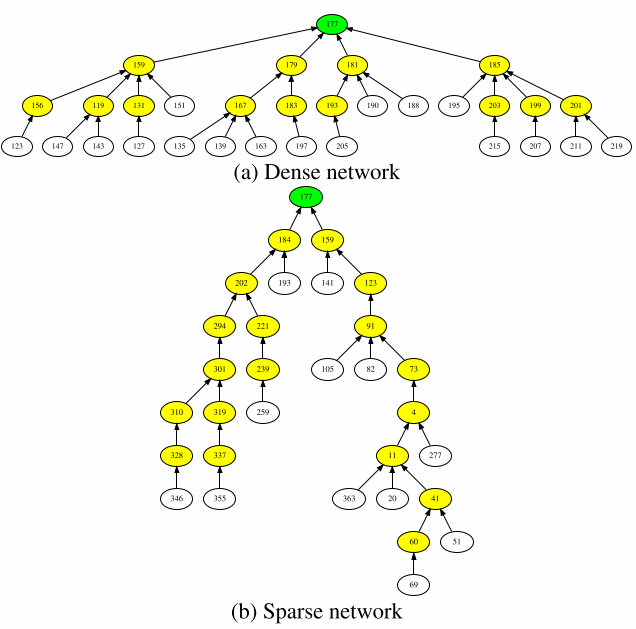
\includegraphics[width=\columnwidth]{topologies_sparse_dense.PNG}
%    \caption{Sparse and dense topology from FIT IoT-lab \cite{EmpiricalSurveyAutonomousElsts2020}}
%    \label{fig_topologies}
%\end{figure}

%Note that this would also not be limited to convergecast, but be applicable to any traffic pattern.

%The proposal should struggle more in dense networks where a node has many neighbors. In those scenarios a node's extra transmissions would have a larger chance of colliding with other nodes extra transmissions (the second challenge mentioned above). Additionally, nodes would have more children, which would leave less room for adding extra transmissions before meeting a RX cell in its schedule (the third challenge). However, it is also in these dense networks where the funneling effect is expected to be the weakest since the network is more shallow. On the contrary, in sparse networks, where the funneling is presumed worse, the mechanism should have equally improved conditions to function.

\section{Open questions}
Which channel selection algorithm should be utilized?

What is the individual contribution of each of the three mechanisms in the proposal?

How does the proposal impact reliability and latency, vs. increased energy consumption? At which limits of the parameters (network density, traffic intensity, etc.) does the proposal provide a benefit, and in which does it not. Or in other words, what are its applications? How does it perform in the scenarios treated by Orchestra/ALICE?

Note that the essence of the proposal is for nodes to opportunistically grab resources. Any gained knowledge from an evaluation, and the proposal itself, is probably generic such that it is applicable to any other scheduling scheme which could accommodate opportunistic extra transmissions.

% needed in second column of first page if using \IEEEpubid
%\IEEEpubidadjcol


% An example of a floating figure using the graphicx package.
% Note that \label must occur AFTER (or within) \caption.
% For figures, \caption should occur after the \includegraphics.
% Note that IEEEtran v1.7 and later has special internal code that
% is designed to preserve the operation of \label within \caption
% even when the captionsoff option is in effect. However, because
% of issues like this, it may be the safest practice to put all your
% \label just after \caption rather than within \caption{}.
%
% Reminder: the "draftcls" or "draftclsnofoot", not "draft", class
% option should be used if it is desired that the figures are to be
% displayed while in draft mode.
%
%\begin{figure}[!t]
%\centering
%\includegraphics[width=2.5in]{myfigure}
% where an .eps filename suffix will be assumed under latex,
% and a .pdf suffix will be assumed for pdflatex; or what has been declared
% via \DeclareGraphicsExtensions.
%\caption{Simulation results for the network.}
%\label{fig_sim}
%\end{figure}

% Note that the IEEE typically puts floats only at the top, even when this
% results in a large percentage of a column being occupied by floats.


% An example of a double column floating figure using two subfigures.
% (The subfig.sty package must be loaded for this to work.)
% The subfigure \label commands are set within each subfloat command,
% and the \label for the overall figure must come after \caption.
% \hfil is used as a separator to get equal spacing.
% Watch out that the combined width of all the subfigures on a
% line do not exceed the text width or a line break will occur.
%
%\begin{figure*}[!t]
%\centering
%\subfloat[Case I]{\includegraphics[width=2.5in]{box}%
%\label{fig_first_case}}
%\hfil
%\subfloat[Case II]{\includegraphics[width=2.5in]{box}%
%\label{fig_second_case}}
%\caption{Simulation results for the network.}
%\label{fig_sim}
%\end{figure*}
%
% Note that often IEEE papers with subfigures do not employ subfigure
% captions (using the optional argument to \subfloat[]), but instead will
% reference/describe all of them (a), (b), etc., within the main caption.
% Be aware that for subfig.sty to generate the (a), (b), etc., subfigure
% labels, the optional argument to \subfloat must be present. If a
% subcaption is not desired, just leave its contents blank,
% e.g., \subfloat[].


% An example of a floating table. Note that, for IEEE style tables, the
% \caption command should come BEFORE the table and, given that table
% captions serve much like titles, are usually capitalized except for words
% such as a, an, and, as, at, but, by, for, in, nor, of, on, or, the, to
% and up, which are usually not capitalized unless they are the first or
% last word of the caption. Table text will default to \footnotesize as
% the IEEE normally uses this smaller font for tables.
% The \label must come after \caption as always.
%
%\begin{table}[!t]
%% increase table row spacing, adjust to taste
%\renewcommand{\arraystretch}{1.3}
% if using array.sty, it might be a good idea to tweak the value of
% \extrarowheight as needed to properly center the text within the cells
%\caption{An Example of a Table}
%\label{table_example}
%\centering
%% Some packages, such as MDW tools, offer better commands for making tables
%% than the plain LaTeX2e tabular which is used here.
%\begin{tabular}{|c||c|}
%\hline
%One & Two\\
%\hline
%Three & Four\\
%\hline
%\end{tabular}
%\end{table}


% Note that the IEEE does not put floats in the very first column
% - or typically anywhere on the first page for that matter. Also,
% in-text middle ("here") positioning is typically not used, but it
% is allowed and encouraged for Computer Society conferences (but
% not Computer Society journals). Most IEEE journals/conferences use
% top floats exclusively.
% Note that, LaTeX2e, unlike IEEE journals/conferences, places
% footnotes above bottom floats. This can be corrected via the
% \fnbelowfloat command of the stfloats package.


%In summary, "\nameref{opp1}" and "\nameref{opp2}" are the most interesting to me. Autonomous scheduling having a %generic focus



% if have a single appendix:
%\appendix[Proof of the Zonklar Equations]
% or
%\appendix  % for no appendix heading
% do not use \section anymore after \appendix, only \section*
% is possibly needed

% use appendices with more than one appendix
% then use \section to start each appendix
% you must declare a \section before using any
% \subsection or using \label (\appendices by itself
% starts a section numbered zero.)
%


%\appendices
%\section{Proof of the First Zonklar Equation}
%Appendix one text goes here.

% you can choose not to have a title for an appendix
% if you want by leaving the argument blank
%\section{}
%Appendix two text goes here.


% use section* for acknowledgment
%\section*{Acknowledgment}


%The authors would like to thank...


% Can use something like this to put references on a page
% by themselves when using endfloat and the captionsoff option.
\ifCLASSOPTIONcaptionsoff
\newpage
\fi


% trigger a \newpage just before the given reference
% number - used to balance the columns on the last page
% adjust value as needed - may need to be readjusted if
% the document is modified later
%\IEEEtriggeratref{8}
% The "triggered" command can be changed if desired:
%\IEEEtriggercmd{\enlargethispage{-5in}}

% references section

% can use a bibliography generated by BibTeX as a .bbl file
% BibTeX documentation can be easily obtained at:
% http://mirror.ctan.org/biblio/bibtex/contrib/doc/
% The IEEEtran BibTeX style support page is at:
% http://www.michaelshell.org/tex/ieeetran/bibtex/
\bibliographystyle{IEEEtran}

% argument is your BibTeX string definitions and bibliography database(s)
\bibliography{IEEEabrv,../../bib/phd_bibtex}

% biography section
%
% If you have an EPS/PDF photo (graphicx package needed) extra braces are
% needed around the contents of the optional argument to biography to prevent
% the LaTeX parser from getting confused when it sees the complicated
% \includegraphics command within an optional argument. (You could create
% your own custom macro containing the \includegraphics command to make things
% simpler here.)
%\begin{IEEEbiography}[{\includegraphics[width=1in,height=1.25in,clip,keepaspectratio]{mshell}}]{Michael Shell}
% or if you just want to reserve a space for a photo:

%begin{IEEEbiography}{Michael Shell}
%Biography text here.
%\end{IEEEbiography}

% if you will not have a photo at all:
%\begin{IEEEbiographynophoto}{John Doe}
%Biography text here.
%\end{IEEEbiographynophoto}

% insert where needed to balance the two columns on the last page with
% biographies
%\newpage

%\begin{IEEEbiographynophoto}{Jane Doe}
%Biography text here.
%\end{IEEEbiographynophoto}

% You can push biographies down or up by placing
% a \vfill before or after them. The appropriate
% use of \vfill depends on what kind of text is
% on the last page and whether or not the columns
% are being equalized.

%\vfill

% Can be used to pull up biographies so that the bottom of the last one
% is flush with the other column.
%\enlargethispage{-5in}

\end{document}
